\cotefile{46}
\scanpage{2}
Schémas en groupes
et fibrés \unsure{principau|principaux}

(Divers)

\mspage{\unsure{1}}

\scanpage{3}
\deleted{\unsure{Groupe fondamental}}

\uline{I}\quad Langage des schémas

\uline{II}\quad Étude élémentaire de \unsure{qqs} classes de morphismes

\uline{III}\quad Cohomologie des faisceaux cohérents.

\uline{IV}\quad Étude locale des morphismes

\uline{V}\quad Étude globale élémentaire des \deleted{quelques} morphismes.
\margin{[N.B. Y inclure propriétés de descente pour morph. \uline{étale}]} 

\uline{VI}\quad Procédés de construction.\deleted{\unsure{1}}

\uline{VII}\quad Schémas en groupes. fibrés principaux (\uline{définition} du \unsure{groupe fondamental})

\uline{VIII}\quad \deleted{Étude \unsure{des schémas} fibrés (\unsure{notions} \illegible{3} \unsure{faisceaux projectifs}; \illegible{3})}
\inserted{Picard et V.A.}

\deleted{\uline{\unsure{IX}}\quad Groupe fondamental}
\margin{$\longleftarrow$ pour la \unsure{coh.} étale\ldots}

\deleted{\uline{\unsure{X}}\quad \unsure{Schémas abéliens}}

\figure{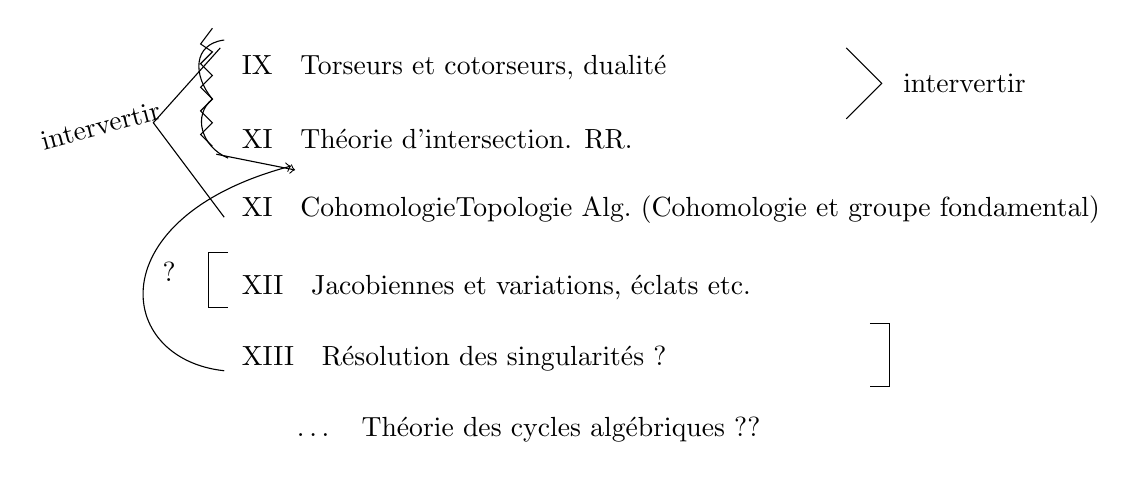
\begin{tikzpicture}[x=1cm,y=1cm]
\node[anchor=west] (ix) at (0,0) {\uline{IX}\quad Torseurs et cotorseurs, dualité};
\node[anchor=west] (x) at (0,-.9) {\uline{X}\deleted{\unsure{I}}\quad Théorie d'intersection. RR.};
\node[anchor=west,align=left] (xi) at (0,-1.8) {\uline{X\unsure{I}}\quad \deleted{\unsure{Cohomologie}}\inserted{\uline{Topologie Alg.}}\ (\deleted{Cohomologie et} groupe fondamental)};
\node[anchor=west] (xii) at (0,-2.8) {\uline{XII}\quad \unsure{Jacobiennes} \unsure{et variations}, \unsure{éclats} etc.};
\node[anchor=west] (xiii) at (0,-3.7) {\uline{XIII}\quad Résolution des singularités ?};
\node[anchor=west] at (.7,-4.6) {\unsure{\ldots}\quad Théorie des cycles \unsure{algébriques} ??};
\draw (-.1,.35) .. controls (-.5,.3) and (-.5,-.1) .. (-.25,-.4)
 .. controls (-.5,-.6) and (-.4,-1) .. (-.05,-1.15);
\draw (-.15,.25)--(-1,-.7)--(-.1,-1.9);
\node[anchor=east,rotate=15] at (-.8,-.5) {\unsure{intervertir}};
\draw[->] (-.2,-1.1)--(.8,-1.3);
\draw[->] (-.1,-3.85) .. controls (-1.5,-3.7) and (-1.7,-1.9) .. (.75,-1.25);
\node at (-.8,-2.6) {?};
\draw (-.05,-2.35)--(-.3,-2.35)--(-.3,-3.05)--(-.05,-3.05);
\draw (8.1,-3.25)--(8.35,-3.25)--(8.35,-4.05)--(8.1,-4.05);
\draw (7.8,.25)--(8.25,-.2)--(7.8,-.65);
\node[anchor=west] at (8.4,-.2) {\unsure{intervertir}};
\draw (-.25,.5)--(-.4,.3)--(-.25,.2)--(-.4,.05)--(-.25,-.1)--(-.4,-.25)--(-.25,-.4)--(-.4,-.55)--(-.25,-.7)--(-.4,-.85)--(-.25,-1);
\end{tikzpicture}}

\mspage{\unsure{2}}

\scanpage{4}
$\unsure{p|\varphi}$-structures des
fibrés vectoriels et
des torseurs.

\mspage{3}

\scanpage{5}
\uline{$\unsure{p|\varphi}$-structures en général.}

1) Soit $\underline S$ un site, $G$ un faisceau en groupes sur $\underline S$,
\[
f:G\longrightarrow G
\]
un endomorphisme. On s'intéresse à la structure
suivante (où, pour $\unsure{\forall}$ torseur $P$ sous $G$,
$P^f$ désigne le torseur déduit par extension du
groupe par $f$) : donnée d'un torseur $P$
sous $G$, et d'un \uline{isom} $P\sim P^f$, ou ce qui
revient au $=$, d'un hom de faisceaux
\[
\varphi:P\longrightarrow P
\]
satisfaisant
\[
\varphi(xg)=\varphi(x)f(g).
\]
Ces objets (au dessus d'objets variables de $S$)
forment un champ\inserted{$\unsure{\Sigma}$ en groupoïdes, avec une section marquée $(G,f)$}.
On se donne des conditions
moyennant lesquelles ce dernier est une gerbe.
Noter que \uline{loc.} un tel $P$ est trivial comme
simple torseur, donc peut s'identifier à $G$ près
à une translation. La structure $\varphi$ est alors
déterminée par la connaissance de $\varphi(1)=a$,
par la formule
\[
\varphi_a(g)=a f(g)
\]
\mspage{4}

\scanpage{6}
et $a$ peut être pris arbitrairement. On voit déjà
que le champ envisagé \uline{couvre}, et il reste
à \deleted{donner}\inserted{voir} la condition moyennant laquelle deux
objets sont tjrs loc isom, ou encore
pour deux éléments $a,b\in G(S)$ $(S\in\underline S)$,
$\varphi_a$ et $\varphi_b$ définissent des objets loc. isom.
Pour ceci, notons que les hom de
$(G,\varphi_a)$ dans $(G,\varphi_b)$ s'identifient aux $u\in G(S)$,
tels que
\deleted{$(G,\varphi_a)\mathbin{\text{---}}$}
\diagram{\begin{tikzcd}
G \arrow[r,no head,"\varphi_a"] \arrow[d,"\rho_u"'] & G \arrow[d,"\rho_u"]\\
G \arrow[r,no head,"\varphi_b"'] & G
\end{tikzcd}}
commute
où $\rho_u(g)=ug$, donc tels que
\[
u a f(g)=b f(ug)\qquad \forall g\in G(S'),\quad S'\text{ sur }S,
\]
ce qui s'écrit aussi simplement
\[
b^{-1}a=f(u)u^{-1}
\]
Donc on trouve que $\Sigma$ \uline{est une gerbe} sss
\uline{l'hom de faisceaux d'ensembles}
\[
u\longmapsto f(u)u^{-1}:G\longrightarrow G
\]
\uline{est un épimorphisme}. Alors $\unsure{\forall}$ objet de
$\Sigma$ est loc isom à $(G,\varphi_e=f)$ lui-$=$,
dont le faisceau des autom. est formé du
sous faisceau des $u$ de $G$ tels que $f(u)u^{-1}=\unsure{11^{-1}|ee^{-1}}=1$,
\mspage{5}

\scanpage{7}
donc le faisceau $N=\operatorname{Ker}(f,\mathrm{id})$ de coïncidence
de $f$ et de $\mathrm{id}_G$. Donc $\Sigma$ \uline{équivaut}
\uline{à la gerbe des $N$-torseurs}.

\textcircled{2}\quad Soit $G$ un schéma en groupes lisse \deleted{connexe} sur le
corps fini $\mathbf F_q$, \inserted{$q=p^n$,} Soit
\[
f=\unsure{\mathrm{fros}|\mathrm{Frob}}^n_{G/k}:G\mathbin{\text{---}}G.
\]
\uline{Théorème} (Lang). L'homomorphisme $u\mapsto f(u)u^{-1}$ de $G$ en
lui-$=$ est \uline{étale}, et \inserted{de plus}\uline{surjectif} (donc couvrant
pour la top. étale) si $G$ est connexe.

Le fait que le morphisme soit \uline{étale} résulte
aussitôt du critère infinitésimal d'étalité, grâce au fait
que \deleted{\unsure{f est}} $\operatorname{Lie}(f)=0$ et grâce au fait que $G$
est lisse (à dégager un lemme). \deleted{De cette façon}
[De cette façon, $N=\operatorname{Ker}(f,\mathrm{id}_G)$ est un groupe étale
\inserted{\unsure{fini}} sur $k$, et
\diagram{\begin{tikzcd}
G/N \arrow[r,"{\text{imm ouvert}}","\varphi"'] & G
\end{tikzcd}}
induit par $f(u)u^{-1}$.]
\deleted{Le morphisme $\varphi$ satisfait}
\inserted{$\boxed{\varphi(gx)=f(g)\varphi(x)g^{-1}}$}
\unsure{Kif-kif} pour $\unsure{\forall}$
morphisme $u\mapsto f(u)g u^{-1}$. On termine, si $G$
est connexe, comme dans Serre Gr. Alg. et corps de classes
p. \unsure{119}.

\margin{\uline{NB} Axiomatique : $G$ \inserted{préschéma en groupes} lisse sur $S$,
$f$ endom. tel que $\operatorname{Lie}(f)=0$.
Alors $u\mapsto f(u)u^{-1}$ est étale, et si $G$ est
à fibres connexes, il est surjectif.}

\mspage{6}

\scanpage{8}
\uline{Corollaire} Soit $S$ sur $\mathbf F_q$. La classification des
torseurs $P$ sous $G_S$, munis de $P\simeq P^f$, i.e
de $\varphi:P\mathbin{\text{---}}P$ satisfaisant $\varphi(xg)=\varphi(x)f(g)$, équivaut
à celle des \deleted{rev. \inserted{étales} \unsure{galoisiens} de $S$, de groupe}
$G(\mathbf F_q)$.

En effet, $N$ est le gr. discret \inserted{sur $k$} (constant)
défini par $G(\mathbf F_q)$, et on applique le n° 1.

\textcircled{3}. Soit $S$ préschéma en car. $p$, et $E$ un
Module (qu. coh.) sur $S$. Une $p$-structure sur $E$
est un hom
\[
\varphi:E^{(p)}\longrightarrow E
\]
[où $E^{(p)}=E\otimes_{\mathcal O_S}(\mathcal O_S,f)$]. La $p$-structure est
dite \uline{non dégénérée} si $\varphi$ est un isom.
On veut classifier les $p$-structures non
dégénérées sur $S$, avec $E$ loc. libre de rang $n$.
Ce sont les structures de $G$-torseurs avec $f$-
rigidification, où $G=\mathrm{GL}(n)_S$, et $f:G\mathbin{\text{---}}G$
est le frobenius. Comme $G$ provient de
$G_0$ sur $\mathbf F_p$, on peut appliquer 2°, on trouve que
\mspage{7}

\scanpage{9}
la classification est celle des torseurs sous
$\mathrm{GL}(n,\mathbf F_p)$, ou ce qui revient au $=$, celle des
faisceaux (ét) en \deleted{groupes} vectoriels sur $\mathbf F_p$, qui
sont loc libres de rang $n$. Si $\unsure{\mathcal L}$ est un
tel faisceau, le Module $E$ qui lui
correspond est simplement
\[
E=\unsure{\mathcal L}\otimes_{\mathbf F_p}\mathcal O_S
\]
[si on note que les faisceaux qu. coh.
(Zar) et les faisceaux qu. coh. ét,
c'est pareil\ldots].

On peut se demander dans quelle mesure les
hypothèses de locale liberté et de type fini sont
nécessaires dans cet énoncé.
\mspage{8}

\scanpage{10}
Frobenius

\mspage{9}

\scanpage{11}
\diagram{\begin{tikzcd}[column sep=small]
& X'^{(p/X)} \arrow[dl] \arrow[ddr] & \\
X' \arrow[d,"p"'] && X' \arrow[ll,"{F_{X'}}"'] \arrow[ul,"{\mathrm{Fr}_{X'/X}}"'] \arrow[d,"p"]\\
X && X \arrow[ll,"{F_X}"']
\end{tikzcd}}
\margin{de car. $p$}

\uline{Proposition}

\uline{On suppose} $p$ \uline{loc. de prés. finie}

1°) Conditions équivalentes

\begin{tabular}{ll}
(i) & $p$ non ramifié\\
(ii) & $\mathrm{Fr}_{X'/X}$ non ramifié\\
(ii bis) & $\unsure{F|\mathrm{Fr}}_{X'/X}$ un monomorphisme
\end{tabular}

2°) Conditions équivalentes

\begin{tabular}{ll}
(i) & $p$ étale\\
(ii) & $\mathrm{Fr}_{X'/X}$ étale\\
(ii bis) & $\mathrm{Fr}_{X'/X}$ un isomorphisme
\end{tabular}

\uline{Dém} 1°) $(\mathrm{ii})\Longleftrightarrow(\mathrm{ii\ bis})$ car monomorphisme $=$ radiciel non ramifié
\margin{17.4.10.}

$(\mathrm{i})\Longleftrightarrow(\mathrm{ii})$ car
\[
\underline\Omega^1_{X'/X}\simeq\underline\Omega^1_{X'/X'^{(p/X)}}
\]

\deleted{\unsure{3}} 2°) $(\mathrm{ii})\Longleftrightarrow(\mathrm{ii\ bis})$ car isom $=$ radiciel surjectif étale

$(\mathrm{i})\Longrightarrow(\mathrm{ii})$ car si $X'$ étale sur $X$, $X'^{(p/X)}$ itou, et
tout $X$-morphisme $X'\mathbin{\text{---}}X'^{(p/X)}$ itou.

$(\mathrm{ii\ bis})\Longrightarrow(\mathrm{i})$. Grâce à 1°) on sait déjà que $X'/X$
est \uline{non ramifié}, donc localement \inserted{(ét)} sur la base
\deleted{\unsure{pour la démo}} c'est une immersion. Donc
on est ramené à ceci : si $X'\mathbin{\text{---}}X$ est
une imm de prés. finie telle que
$X'\longrightarrow X'^{(p/X)}$ un isom, alors c'est une imm.
ouverte. On peut supposer que c'est
une imm fermée définie par Idéal $\mathcal J$
de type fini, alors $X'^{p/X}$ est défini
par l'Idéal $\unsure{\mathcal J^p}$, l'hyp. s'écrit $\mathcal J=\unsure{\mathcal J^p}$,
ce qui implique que \deleted{\unsure{l'immersion}} $X'\mathbin{\text{---}}X$ est
une imm ouverte (16.1.8), O.K.
\mspage{10}

\scanpage{12}
\uline{Frobéniuseries.}

On désigne par $(\mathrm{Sch})_p$ \inserted{$=(\mathrm{Sch})_{/\operatorname{Spec}(\mathbf Z/p\mathbf Z)}$} la sous catégorie pleine des $(\mathrm{Sch})$
formée des préschémas de car. $p$, et tous les préschémas
envisagés sont de car. $p$.

On définit un hom fonctoriel en $X$
\[
\operatorname{Frob}(X):X\longrightarrow X
\]
\margin{\figure{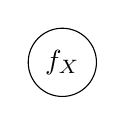
\begin{tikzpicture}\node[draw,circle] {$f_X$};\end{tikzpicture}}}
[\uline{Frobenius absolu}] par la condition d'être l'identité
sur les espaces topologiques, et $f\mapsto f^p$ sur les
fonctions.

Soit $S$ fixé. Pour tout $X$ sur $S$, on a donc
un carré commutatif
\diagram{\begin{tikzcd}
X \arrow[r,"{\operatorname{Frob}(X)}"] \arrow[d,"f"'] & X \arrow[d,"f"]\\
S \arrow[r,"{\operatorname{Frob}(S)}"'] & S
\end{tikzcd}}
\margin{\diagram{\begin{tikzcd}
X \arrow[r,"{\mathrm{Fr}_{X/S}}"] & X^{(p/S)}
\end{tikzcd}}}
\margin{Changer les flèches horizontales \unsure{de direction}}
(où $f$ est le morphisme structural). \deleted{Ainsi}, Posons
\[
\deleted{\unsure{F}}P_S(X)=X\times_S(S,\operatorname{Frob}(S)):
\]
\margin{\figure{\begin{tikzpicture}
\node[draw,ellipse] {$X^{(p/S)}$ ou $X^{(p/f)}$ ou $X^{(p)}$};
\node[anchor=north west] at (-2.1,-.35) {$(X/S)^{(p)}$};
\end{tikzpicture}}}
$\unsure{p_S|P_S}(X)$ est un foncteur
\[
P_S:(\mathrm{Sch})_{/S}\longrightarrow(\mathrm{Sch})_{/S}
\]
\margin{dire que $X\longrightarrow P_S(X)$ est un \uline{homéomorphisme}\deleted{\unsure{étale}} \uline{universel}.}
qui étant un foncteur de changement de base, en
a toutes les propriétés [commute aux
$\varprojlim$, aux sommes, transforme type fini
\mspage{11}

\scanpage{13}
resp. séparé resp... en type fini \unsure{resp.} séparé resp...]

Le carré précédent nous donne un $S$-homomorphisme
fonctoriel en $X$
\[
\operatorname{Frob}_S(X):X\longrightarrow p_S(X)
\]
\margin{\figure{\begin{tikzpicture}\node[draw,ellipse] {$\mathrm{Fr}_{X/S}$};\end{tikzpicture}}}
[et $\operatorname{Ver}_S(X):p_S(X)\longrightarrow X$
compatible à $\operatorname{Frob}(S)$]
\margin{\diagram{\begin{tikzcd}[column sep=small]
X \arrow[r,"{\operatorname{Frob}_S(X)}"] \arrow[rr,bend left=35,"{\operatorname{Frob}(X)}"] & p_S(X) \arrow[r,"\mathrm{pr}_1"] \arrow[d] & X \arrow[d]\\
& S \arrow[r,"{\operatorname{Frob}(S)}"'] & S
\end{tikzcd}}}

Définitions analogues pour un Module $E$
sur $X$, on pose
\[
p_S(E)=E\otimes_{\mathcal O_X}\mathcal O_{p_S(X)}
=E\otimes_{\mathcal O_S}(\mathcal O_S,\operatorname{Frob}(S)),
\]
\[
\deleted{=\unsure{E}}
\]
\inserted{C'est un foncteur en les $\mathcal O_X$-Modules $\underline E$, \deleted{\unsure{d'un homom.}}}
\deleted{$\operatorname{Frob}(\underline E):p_S(\underline E)\longrightarrow\underline E$}

En particulier pour $X=S$, on trouve
\[
p_S(\underline E)=E\otimes_{\mathcal O_S}(\mathcal O_S,\operatorname{Frob}(S))
\]
\margin{Rôle universel de $E^{(p)}=p_S(\underline E)$}
On laisse aussi tomber $S$ dans cette dernière formule, et on pose parfois
$p(E)$.
\margin{\unsure{Isom. can.} (\unsure{transitivité} de l'extension de la base)
$p(E)\simeq\operatorname{Frob}_S(X)^*(p_S(\underline E))$}
Il rentre dans les propriétés générales du changement de base, que si
$\deleted{p_S(\underline E)}\inserted{\underline E}$ est
\unsure{quasi-cohérent} (resp. \deleted{\unsure{de}} qu. coh. de type fini,
qu. coh. de présentation finie, plat etc) il en est de même de
\deleted{$\unsure{\underline E}$} $p_S(\underline E)$.
Le foncteur $\underline E\rightsquigarrow p_S(\underline E)$ est exact à droite, commute
\deleted{(\unsure{est un} \illegible{2})}
à $\otimes$, mais en général n'est pas exact à gauche et ne commute pas à Hom.
\figure{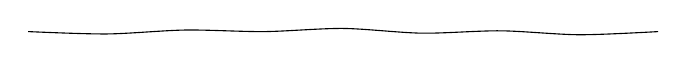
\begin{tikzpicture}\draw plot[smooth] coordinates {(0,0) (1,-.03) (2,.02) (3,0) (4,.04) (5,-.02) (6,.01) (7,-.04) (8,0)};\end{tikzpicture}}
\mspage{12}

\scanpage{14}
Si $E=A$ est une Algèbre qu. coh.\inserted{(\unsure{resp. et graduée})}, il
en est de même de $p_S(A)$, et on aura
\[
\left\{\begin{aligned}
p_S(\operatorname{Spec}(A))&=\operatorname{Spec}(p_S(A))\\
p_S(\operatorname{Proj}(A))&=\operatorname{Proj}(p_S(A))
\end{aligned}\right.
\]
\margin{\diagram{\begin{tikzcd}[column sep=small,row sep=small]
& p_S(X') \arrow[r] \arrow[d] & X' \arrow[d]\\
X \arrow[r] \arrow[dr,"f"'] & p_S(X) \arrow[r] \arrow[d] & X \arrow[d,"f"]\\
& S \arrow[r,"{\operatorname{Frob}(S)}"'] & S
\end{tikzcd}}}
et les hom $\operatorname{Frob}_S(X)$ pour $X=\operatorname{Spec}(A)$,
resp. $X=\operatorname{Proj}(A)$ sont ceux déduits de
$\operatorname{Frob}_S(A):p_S(A)\longrightarrow A$, grâce à
la puissance \unsure{$p$ième}. (\unsure{$q$ième}).

Corollaires :

\deleted{Exemples : $E=\underline{\mathcal O}$}
\[
\left\{\begin{aligned}
p_S(\underset{\sim}{\mathrm V}(\underline E))&=\underset{\sim}{\mathrm V}(p_S(\underline E))\\
p_S(\underset{\sim}{\mathrm P}(\underline E))&=\underline{\mathrm P}(p_S(\underline E))
\end{aligned}\right.
\]
les hom de Frobenius pour les précédents sont ceux associés à
\deleted{$p_S(E)\quad\operatorname{Frob}_S(\underline E):p_S(\underline E)\longrightarrow\underline E$}.
\deleted{\unsure{grâce à hom}}
\[
\underline E^{(p)}\longrightarrow\operatorname{Symm}^p(\underline E)\subset\operatorname{Symm}(\underline E)
\]
déduit de l'élévation à la puissance \unsure{$p$ième}.
\margin{\diagram{\begin{tikzcd}[column sep=small,row sep=large]
X' \arrow[r,"{\operatorname{Frob}_X(X')}"] \arrow[rr,bend left=30,"{\operatorname{Frob}_S(X')}"] \arrow[dr,"g"'] & p_X(X') \arrow[r,"\unsure{r}"] \arrow[d] & p_S(X') \arrow[r] \arrow[d] & X' \arrow[d,"g"]\\
& X \arrow[r,"{\operatorname{Frob}_S(X)}"] \arrow[rr,bend right=18,dashed,"{\operatorname{Frob}(X)}"'] \arrow[dr,"f"'] & p_S\deleted{\unsure{f}}(X) \arrow[r] \arrow[d] & X \arrow[d,"f"]\\
&&S \arrow[r,"{\operatorname{Frob}(S)}"'] & S
\end{tikzcd}}
trois carrés cartésiens}
\margin{\figure{\begin{tikzpicture}
\draw (0,-2.5) .. controls (-.3,-1.4) and (-.05,-.7) .. (-.45,-.5)
.. controls (-.1,-.35) and (-.45,.3) .. (0,1);
\draw[->] (-.45,-.5) .. controls (-.5,1) and (-.5,6) .. (-.45,7)
.. controls (-.45,7.6) and (.3,7.8) .. (.45,8.1);
\end{tikzpicture}}}
[N.B. la structure vectorielle de $\mathrm V(\underline E)$ n'est
pas conservée, mais bien entendu la structure en
groupe est conservée. Noter que dans l'hom de
Frobenius $\underset{\sim}{\mathrm P}(\underline E)\longrightarrow
p_S(\underset{\sim}{\mathrm P}(\underline E))=\underset{\sim}{\mathrm P}(p_S(\underline E))$, corres\unsure{.}
\mspage{13}

\scanpage{15}
un hom d'Algèbres graduées
\[
\operatorname{Symm}\underline E\longrightarrow(\operatorname{Symm}E)_{(p)}
\]
(degrés multipliés de $p$)

Le \deleted{\unsure{f}} faisceau inverse de
$\underline{\mathcal O}_{\underset{\sim}{\mathrm P}(p_S(\underline E))}(1)$ est
$\underline{\mathcal O}_{\underset{\sim}{\mathrm P}(\underline E)}(p)$.
\unsure{Le noter. cas plus général}.

Si $\unsure{\underline L|\underline E}$ est un Module \uline{inversible}, on a un
\uline{isom canonique}
\[
p(\underline L)\simeq\underline L^{\otimes p}.
\]
\margin{Exemple : $\underline E=\mathcal O_S^n$, d'où
$\deleted{p_S(\unsure{\mathrm V}(\underline E))}p_S(\underline E)\simeq\mathcal O_S^n$, donc
$p_S(S[t_1,\ldots,t_n])\simeq S[t_1,\ldots,t_n]$, l'hom canonique
défini par $t_i\rightsquigarrow t_i^p$.
Si on a un sous-schéma de $\underline E$ défini par des équations,
on élève les \uline{coefficients} de ces équations à la puissance \unsure{$p$ième}.
Analogue pour des équations homogènes, \unsure{et} définissant un schéma projectif.}
\figure{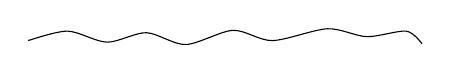
\begin{tikzpicture}\draw plot[smooth] coordinates {(0,0) (.5,.12) (1,-.02) (1.5,.1) (2,-.05) (2.6,.13) (3.1,0) (3.8,.15) (4.3,.05) (4.8,.12) (5,-.04)};\end{tikzpicture}}

Changement de base des Frobenius

\deleted{[cf diagramme]}

1°) (cf diagramme)
\[
\unsure{P_X|p_X}(X')\simeq p_S(X')\times_{p_S(X)}(X,\operatorname{Frob}_S(X)):
\]
et avec cette identification, \deleted{\unsure{un}}
$\operatorname{Frob}_X(X')$ est défini de façon évidente par
$\operatorname{Frob}_S(X')$ et $\operatorname{Frob}_S(X)\circ g$.

2°) Si on a un chgt de base $S'\mathbin{\text{---}}S$, on a
\[
p_S(X)\times_S S'\simeq p_{S'}(X\times_S S')
\]
Cet isom étant fonctoriel en $X$, \deleted{\unsure{et le foncteur}}
\inserted{\unsure{le foncteur chgt}}
\unsure{l'hom de ch. de base} transforme $\operatorname{Frob}_S(X)$ en
$\operatorname{Frob}_{S'}(X\times_S S')$.
\mspage{14}

\scanpage{16}
\figure{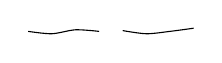
\begin{tikzpicture}\draw plot[smooth] coordinates {(0,0) (.3,-.03) (.6,.02) (.9,0)};\draw plot[smooth] coordinates {(1.2,.01) (1.5,-.03) (1.8,0) (2.1,.04)};\end{tikzpicture}}
Frobénius itéré : notation $p_S^\nu(X)$, $\operatorname{Frob}_S^\nu(X)$.
Les développements précédents sont valables, en \unsure{changeant} les
puissances \unsure{$p$ième} par les puissances $p^\nu$-ièmes.
\figure{\begin{tikzpicture}\draw plot[smooth] coordinates {(0,0) (.3,.07) (.6,-.01) (.9,0)};\draw (1.2,.02) .. controls (1.4,-.03) .. (1.7,0);\draw (1.9,.03)--(2,.0);\draw (2.3,.02)--(2.4,0);\end{tikzpicture}}

Cas d'un préschéma de \uline{base parfait}.
On dira que $S$ est \uline{parfait} si \deleted{\unsure{son}}
$\mathcal O_S\mathbin{\overset{\operatorname{Frob}(S)^*}{\text{---}}}\mathcal O_S$
est un \uline{isomorphisme}.
Le cas le plus important est celui où $S$ est le spectre d'un corps, où
la terminologie coïncide avec celle usuelle.

\uline{Dans ce cas}, \uline{le préschéma} $p_S^\nu(X)$ est
\uline{isom au préschéma} $X$ \uline{par} $\mathrm{pr}_1$, \uline{mais}
\uline{on se rappellera que ce n'est pas un} $S$-\uline{isom}.
\uline{En général}, $p_S^\nu(X)$ \uline{n'est pas}
$S$-\uline{isom à} $X$.
\figure{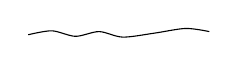
\begin{tikzpicture}\draw plot[smooth] coordinates {(0,0) (.3,.05) (.6,-.02) (.9,.04) (1.2,-.03) (1.6,.02) (2,.08) (2.3,.04)};\end{tikzpicture}}

Cas d'un corps de base fini, à $q=p^{\unsure{h|\nu}}$ éléments.
\inserted{$[\deleted{\unsure{\nu=h\nu}}\unsure{\nu\mapsto h\nu}]$}
Alors $\operatorname{Frob}_{\unsure{S}}^{h\nu}(S):S\longrightarrow S$
est l'identité. Donc \uline{pour de tels} $\nu$,
\deleted{\unsure{le} \illegible{2}}\inserted{le morphisme can}
$p_S^\nu(\unsure{X})\mathbin{\text{---}}X$ \uline{est un} $S$-\uline{isom}.
Donc on peut considérer $\operatorname{Frob}_S^{h\nu}(X)$ comme un
\mspage{15}

\scanpage{17}
endomorphisme de $X$, qui n'est d'ailleurs autre que
$(\operatorname{Frob}_S^\nu(X))^k$, comme on constate aussitôt.

D'ailleurs, dans le cas où $\unsure{h|\nu}=1$, i.e.
sur la base absolue $\mathbf Z/p\mathbf Z$, on trouve que
$\operatorname{Frob}_{\mathbf Z/p\mathbf Z}(X)$ est le Frobenius absolu du début.

\uline{Corollaire} Si $S$ est sur $\mathbf F_q$, et si $X$ provient d'un
\unsure{schéma} \deleted{\unsure{sur}} $\mathbf F_q$ \uline{par extension} de la base...
\figure{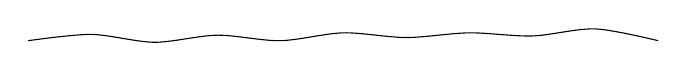
\begin{tikzpicture}\draw plot[smooth] coordinates {(0,0) (.8,.08) (1.6,-.02) (2.4,.07) (3.2,0) (4,.1) (4.8,.04) (5.6,.1) (6.4,.06) (7.2,.15) (8,0)};\end{tikzpicture}}

\uline{Cas des groupes}. Si $G$ est muni d'une
structure algébrique définie sur $S$, il en est
de même de $p_S(G)$, et \deleted{$\operatorname{Frob}_S(X)$}
\[
\operatorname{Frob}_S^\nu(G):G\longrightarrow p_S^\nu(G)
\]
est un morphisme pour les structures en question.
Considérons son noyau, noté
\[
U_\nu(G)=\operatorname{Ker}(\operatorname{Frob}_S^\nu(G)).
\]
\margin{C'est le plus grand sous-schéma en groupes $U\unsure{\subset}G$
pour lequel $\operatorname{Frob}^{\nu}\mathrm{abs}$ est \unsure{trivial}.}
\deleted{\uline{Proposition} Si $G$ est de présentation finie sur $S$, alors
\unsure{?} $U_\nu(G)$ est de présentation finie et \deleted{\unsure{de}}
fini \deleted{\unsure{un}} radiciel \inserted{(surjectif)} sur $S$.}
\mspage{16}

\scanpage{18}
\uline{Lemme 1} Un morphisme \deleted{radiciel surjectif}\inserted{de préschémas}
$f:T\mathbin{\text{---}}S$ qui est un homéomorphisme \unsure{sur|uni}
\deleted{\unsure{universel}} est affine.
\margin{\figure{\begin{tikzpicture}\draw (0,0)--(0,-1.1);\end{tikzpicture}}}

\deleted{En effet, \unsure{c'est} un homéomorphisme, il est
quasi-compact, Étant radiciel, il est séparé, donc
\deleted{$f_*(\mathcal O_T)=A$ est quasi-cohérent}
\inserted{pour tout $F$ sur $T$, $f_*(F)$ est} quasi-cohérent.
Supposons $S$ \deleted{affine, \unsure{prenons, pour voir les} $F$ qu. coh. sur $T$}
On peut supposer $S$ affine, donc quasi-compact, donc $T$ est quasi-compact.
On a donc $T=\bigcup_i T_i$, réunion \unsure{finie}
d'ouverts affines; \deleted{et $T_i$ est} comme
$f(T_i)$ est ouvert de $S$, il est réunion d'ouverts affines $S_{ij}$,
\deleted{\unsure{dont chacun}}
\inserted{et $T_i=\bigcup_j T_{ij}$, où $T_{ij}=f^{-1}(S_{ij})=f_i^{-1}(S_{ij})$}
est affine.
\deleted{$T=\bigcup_{ij}f^{-1}(S_{ij})$}
comme $T$ est quasi-cpt, $T$ est réunion finie}

On peut supposer $S$ \uline{affine}.
Soit $s\in S$, alors $f^{-1}(s)$ est réduit à un pt,
donc admet un voisinage affine $U$.
Comme $f(U)$ est un voisinage de $s$, il contient un
\uline{voisinage} affine $V$ de $s$. Alors on a
\[
f^{-1}(V)=f'^{-1}(V)
\]
où $f':U\mathbin{\text{---}}S$ est induit par $f$.
Comme $f'$ est un morphisme de schémas affines, et
$V$ est affine, $f'^{-1}(V)$ l'est, O.K.
\mspage{17}

\scanpage{19}
\uline{Proposition 2} Soit $G$ un schéma en groupes sur $S$.
Pour qu'il soit d'ordre infinitésimal $\nu$, i.e.
$U_\nu(G)=G$, il f. et s. que $G$ soit \uline{affine} sur $S$, et défini
par une Algèbre augmentée $A$
\deleted{[à \unsure{comultiplication} \unsure{diagonale donnée}]}
\deleted{\inserted{et tel que $x\in I\unsure{\Rightarrow}x^{p^\nu}=0$}}
dont l'\uline{I}déal d'augmentation \deleted{est de}
\inserted{a tous les éléments de} puissances $p^\nu$-ièmes nulles.
D'autre part, pour $G$ quelconque, $U_\nu(G)$ est
\deleted{can. isomorphe}\inserted{identique}
au voisinage infinitésimal d'ordre $p^\nu$ de la section unité.
\margin{N.B. Ne fait intervenir que la section marquée de $G$,
et pas la structure de groupe}
\mspage{18}

\scanpage{20}
Détermination de ${}_p\operatorname{Pic}(X)$, $X$ propre normal sur $k$ parfait de car. $p$.

On aura ${}_p\operatorname{Pic}(X)={}_pH^1(X,\underline{\mathcal O}_X^*)$

Comme $X$ est \uline{réduit}, on a une suite exacte
\diagram{\begin{tikzcd}
0 \arrow[r] & \underline{\mathcal O}_X^* \arrow[r,"{x\to x^p}"] & \underline{\mathcal O}_X^* \arrow[r] & \underline{\mathcal O}_X^*/\underline{\mathcal O}_X^{*p} \arrow[r,no head] & 0
\end{tikzcd}}
d'où par la suite exacte de cohomologie, pour $A=H^0(X,\underline{\mathcal O}_X)$
\diagram{\begin{tikzcd}[column sep=small]
0 \arrow[r] & A^* \arrow[r,"{x\rightsquigarrow x^p}"] & A^* \arrow[r] & \Gamma(X,\underline{\mathcal O}_X^*/\underline{\mathcal O}_X^{*p}) \arrow[r] & {}_pH^1(X,\underline{\mathcal O}_X^*) \arrow[r] & 0
\end{tikzcd}}
et comme $X$ est réduit et propre sur $k$, donc $A$ réduit
fini \deleted{et séparable} sur $k$, et $k$ parfait, on aura
$A^*\simeq A^{*p}$, d'où
\[
{}_p\operatorname{Pic}(X)\simeq\Gamma(X,\underline{\mathcal O}_X^*/\underline{\mathcal O}_X^{*p})
\]
\margin{($X$ réduit et propre sur $k$ parfait)}
Considérons l'hom de dérivation logarithmique
\[
\underline{\mathcal O}_X^*\longrightarrow\Omega^1_{X/k}\qquad
f\rightsquigarrow\frac{df}{f}
\]
elle est nulle sur $\underline{\mathcal O}_X^{*p}$, donc on a un hom
\[
\underline{\mathcal O}_X^*/\underline{\mathcal O}_X^{*p}\longrightarrow
\underbrace{Z\Omega^1_{X/k}}_{\text{formes fermées}}
\]
Cet hom est-il injectif? Noter que si $K$ est l'anneau
des fonctions rationnelles sur $X$, alors $f\in K$, $df=0$
$\Rightarrow f\in K^p$ [car \deleted{$K$} on est ramené au cas où $K$
est un corps, et $K$ \deleted{est libre sur} a alors une
$p$-base sur $K^p\supset k$...]. Or $X$ étant \uline{normal}, si $f\in\mathcal O_X$ est
\mspage{19}

\scanpage{21}
tel que $df=0$, \inserted{donc $f\in K^{*p}$}, on a
$f\in\underline{\mathcal O}_X^p$.
\inserted{[$\underline{\mathcal O}_X^*/\underline{\mathcal O}_X^{*p}\longrightarrow
\mathcal R_X^*/\mathcal R_X^{*p}$ est injectif]}
Donc $X$ \uline{étant normal}, on a un hom \uline{injectif}
\diagram{\begin{tikzcd}
0 \arrow[r] & \underline{\mathcal O}_X^*/\underline{\mathcal O}_X^{*p} \arrow[r] & Z\underline\Omega^1_{X/k}
\end{tikzcd}}
D'après Cartier, un élément dans l'image est tel que
$C\omega=\omega$ [$C$ l'opération de Cartier], et du pt de
vue birationnel la réciproque est vraie : si $\omega$ est une
1-forme fermée telle que $C\omega=\omega$, alors $\omega=\dfrac{df}{f}$,
où $f$ est une \uline{fonction rationnelle} qui n'est nulle
sur aucun \unsure{composant|composante} de $X$,
\deleted{D'ailleurs, comme}\inserted{déterminée mod} $K^{*p}$.
Comme $\underline{\mathcal O}_X^*/\underline{\mathcal O}_X^{*p}\longrightarrow
\underline{\mathcal R}_X^*/\underline{\mathcal R}_X^{*p}$ est injectif,
pour montrer que $\omega$ provient d'une section de
$\underline{\mathcal O}_X^*/\underline{\mathcal O}_X^{*p}$, la question est \uline{locale},
donc il faut prouver que si $f\in(K=\text{corps des fractions de }\mathcal O)^*$,
telle que $\dfrac{df}{f}$ \uline{régulière}, alors $f=g^p h$, avec $h\in\mathcal O^*$,
i.e. \deleted{un diviseur} l'hom
\[
\mathcal R_X^*/\underline{\mathcal O}_X^*\longrightarrow
\underline\Omega^1_{\unsure{k}}(\underline K)/\underline\Omega^1(\underline{\mathcal O}_X)
\]
est \uline{injectif}. $X$ étant normal, \deleted{donc régulier en \unsure{codim 1}},
on est ramené au cas où $X$ est \deleted{\unsure{non}} régulier ...
\mspage{20}

\scanpage{22}
\uline{Pb}\qquad $X$ sur $S$ en car $p>0$

a) Définir une opération ``tensorielle''
$\mathcal O_X$-linéaire
\[
\underline\Omega^1_{X/S}\longrightarrow
?\deleted{\unsure{\operatorname{Symm}}^p}(\Omega^1_{X/S})
\]
qui soit transposée dans un sens convenable
de \deleted{$\unsure{\partial}$} $\partial\mathbin{\text{---}}\partial^p$
sur les $S$-dérivations, et compatible avec les carrés
\diagram{\begin{tikzcd}
X \arrow[d] & X' \arrow[l] \arrow[d]\\
S & S' \arrow[l]
\end{tikzcd}}

Il faudrait que lorsque $\omega$ est une forme \uline{fermée},
on trouve quelque chose dans
$\deleted{\unsure{\operatorname{Symm}}^p_{\mathcal O_X}}\boxed{\underline\Omega^1_{X/S}{}^{(p)}}$
(puissance Frobéniusienne de $\underline\Omega^1_{X/S}$),
ce qui est l'opération de Cartier.
Si les $\omega_i$, $\partial_j$ sont tels que
\unsure{on n'en sort pas} par $d$, $[\ ,\ ]$, et que
les produits scalaires $\langle\omega_i,\partial_j\rangle$ sont des c\textsuperscript{tes},
on voit qu'on doit \unsure{échouer|aboutir} dans
$\boxed{\operatorname{Symm}^p(\underline\Omega^1_{X/S})}$.

b) Montrer qu'un groupe infinitésimal d'ordre $1$ sur $S$
est défini par $\Omega$ qu. coh. sur $S$, avec
\[
C:\Omega\longrightarrow\operatorname{Symm}_{\mathcal O_S}^p(\Omega)
\]
\[
d_1:\Omega\mathbin{\text{---}}\bigwedge_{\mathcal O_S}^2\Omega
\]
\margin{\unsure{satisfaisant} certaines équations.}
\margin{Dire que $G$ est commutatif signifie que $d_1=0$.}
\margin{c) Définir le ``Verschiebung'' $V_S(X):p_S(G)\mathbin{\text{---}}G$
pour un schéma en groupes comm. $G$ sur $S$.}
\mspage{21}

\scanpage{23}
\margin{n\textsuperscript{o}329}
\uline{CHAPITRE II}

\figure{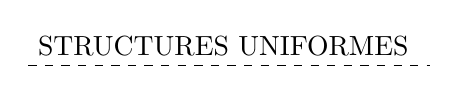
\begin{tikzpicture}\node[anchor=south west] at (0,0) {STRUCTURES UNIFORMES};\draw[dashed] (0,0)--(5.1,0);\end{tikzpicture}}

1. Espaces uniformes.

\uline{1. Définition d'une structures uniforme.}

DEFINITION 1. \uline{Etant donné un ensemble} $X$, \uline{on dit qu'un ensemble} $\underline U$ \uline{de parties de}
$X\times X$ \uline{définit sur} $X$ \uline{une structure uniforme s'il satisfait aux axiomes}
$(F_{\mathrm I})$ \uline{et} $(F_{\mathrm{II}})$ \uline{du chap.} I, 3\textsuperscript{e} éd., § 6, n\textsuperscript{o}1, \uline{et aux axiomes suivants} :

$(U_{\mathrm I})$\quad \uline{Tout ensemble de} $\underline U$ \uline{contient la diagonale} $\Delta$ (fig.2).

$(U_{\mathrm{II}})$\quad \uline{La relation} $V\in\underline U$ \uline{entraîne} $V^{-1}\in\underline U$.

$(U_{\mathrm{III}})$\quad \uline{Quel que soit} $V\in\underline U$, \uline{il existe} $W\in\underline U$ \uline{tel que} $W\circ W\in V$.

\uline{On dit que les ensembles de} $\underline U$ \uline{sont les entourages de la structures uniforme définie sur} $X$ \uline{par} $\underline U$.

Si $V$ est un entourage d'une structure uniforme sur $X$, on conviendra de
considérer la phrase ``x et y sont voisins d'ordre V'' comme une relation équivalente à $(x,y)\in V$.

\uline{Remarques.}-- 1) Pour rendre le langage plus imagé, on pourra employer
les expressions ``x et y sont assez voisins'' et ``x et y sont aussi
voisins qu'on veut'' dans certains énoncés. Par exemple, on dira
qu'une relation $R\{x,y\}$ est vérifiée \uline{si x et y sont assez voisins},
lorsqu'il existe un entourage $V$ tel que la relation $(x,y)\in V$ \uline{entraîne} $R\{x,y\}$.

2) La conjonction des axiomes $(U_{\mathrm{II}})$ et $(U_{\mathrm{III}})$ est (compte tenu des autres axiomes des structures uniformes) équivalente à l'axiome.

$(U_a)$\quad \uline{Quel que soit} $V\in\underline U$, \uline{il existe} $W\in\underline U$ \uline{tel que} $W\unsure{\circ}W^{-1}\in V$.

Il est clair en effet que $(U_{\mathrm{II}})$ et $(U_{\mathrm{III}})$ entraînent $(U_a)$. Inversement, si $(U_a)$ est vérifié, on a $W^{-1}=\Delta\circ W^{-1}\subset V$ d'après $(U_{\mathrm I})$ ;
\mspage{22}

\scanpage{27}
\mspage{-4}
\diagram{\begin{tikzcd}[column sep=large,row sep=large]
G & & G^p \arrow[ll,"\mu"'] \arrow[dl,"i"'] & & G \arrow[ll,"\delta"'] \arrow[ddll,"F"] \\
& \Sigma^pG \arrow[ul,"a"] & & & \\
& & G^{\deleted{\unsure{p}}\inserted{(p)}} \arrow[ul,"r"'] & &
\end{tikzcd}}

où $\delta$ est l'application diagonale et $\mu$ l'application $(g_1,\ldots,g_p)\dashrightarrow g_1+\cdots+g_p$; $\Sigma^pG$ est le produit symétrique de G (voir Serre, loc. cit.) ; $(i,a)$ est la décomposition canonique de $\mu$ ; quant à la décomposition $i.\delta=r.F$, elle est définie de façon canonique pour toute variété algébrique (voir Serre, loc.cit.).

Le diagramme ci-dessus est donc défini pour tout groupe algébrique commutatif, affine ou non. On posera donc $V=a.r$ et on aura $V.F=p$.
\mspage{26}

\scanpage{28}
\uline{\unsure{Frobéniuseries}}

\uline{pour faisceaux}

\uline{étales}
\mspage{27}

\scanpage{29}
\deleted{\boxed{\deleted{\unsure{I}}X}\quad Sous-groupes \unsure{des} \unsure{fibres|tores}

des schémas en

gr. \unsure{sur} \unsure{affines}

\unsure{et} \unsure{simples} $/S$}
\mspage{28}

\scanpage{30}
\uline{\unsure{Reprenons}}

Considérons un préschéma $X/\mathbf F_p$, et
\diagram{\begin{tikzcd}X & X \arrow[l,"\operatorname{Fr}_X"']\end{tikzcd}}
Comme $\operatorname{Fr}_X$ est un homéo. univ. on conclut que pour un faisceau $F$ sur $X$ et un faisceau $G$ sur $X$ (pour top étale), la donnée de
\diagram{\begin{tikzcd}G \arrow[r,"\alpha"] & \operatorname{Fr}_X^*(F)\end{tikzcd}}
\uline{équivaut} à la donnée de
\diagram{\begin{tikzcd}\operatorname{Fr}_{X*}(G) \arrow[r,"\beta"] & F\end{tikzcd}}
(car $\operatorname{Fr}_{X*}$ et $\operatorname{Fr}_X^*$ sont \inserted{ici} des foncteurs adjoints du côté inhabituel).

Ainsi, la donnée de $\alpha$ définit
\diagram{\begin{tikzcd}\operatorname{Fr}_{X*}(G) \arrow[r,"\operatorname{Fr}_{X*}(\alpha)"] & \operatorname{Fr}_{X*}\operatorname{Fr}_X^*(F) \arrow[r,leftrightarrow,"\sim","\mathrm{can}^{-1}" above,yshift=1ex] & F\end{tikzcd}}
et inversement la donnée de $\beta$ définit
\diagram{\begin{tikzcd}G \arrow[r,no head,"\sim","\mathrm{can}^{-1}" above,yshift=1ex] & \operatorname{Fr}_X^*\operatorname{Fr}_{X*}(G) \arrow[r,"\operatorname{Fr}_X^*(\beta)"] & \operatorname{Fr}_X^*(F)\end{tikzcd}}
Nous allons \uline{\unsure{fabriquer}} \deleted{\unsure{donc}} des hom qui se correspondent de cette façon\textsuperscript{*} \deleted{et} Nous allons maintenant, pour $F=G$, définir \deleted{\unsure{des}} un hom canonique
\margin{\textsuperscript{*} \unsure{en mettant les barres sur} $\unsure{*}$ \unsure{et} $\unsure{*}$ \unsure{pour distinguer} \unsure{à la fois} \unsure{opérations}.}
\margin{\figure{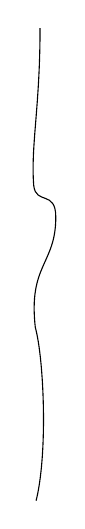
\begin{tikzpicture}[x=1cm,y=1cm]\draw (0,0)..controls(0,-1)and(-.12,-1.5)..(-.08,-2)..controls(-.05,-2.25)and(.2,-2.05)..(.2,-2.4)..controls(.2,-3)and(-.15,-3)..(-.06,-3.8)..controls(.05,-4.2)and(.1,-5.4)..(-.05,-6);\end{tikzpicture}}}
\diagram{\begin{tikzcd}[column sep=large]
(1)\quad F & \operatorname{Fr}_X^*(F) \arrow[l,"\operatorname{Fr}_{F/X}"'] \arrow[l,phantom,"\deleted{\unsure{\rightarrow}}" description]
\end{tikzcd}}\qquad i.e.
\diagram{\begin{tikzcd}[column sep=large]
(2)\quad\operatorname{Fr}_{X*}(F) \arrow[r,"\operatorname{Fr}_{F/X}"] & F
\end{tikzcd}}
(qui est d'ailleurs un isom, mais on voudra l'ignorer dans la plupart des cas !). C'est sous la forme (2) que la définition \unsure{faiscea-}
\mspage{29}

\scanpage{31}
\unsure{tique} est la plus évidente. Car, si $U$ est étale sur $X$
\[
\operatorname{Fr}_{X*}(F)(U)=F(\operatorname{Fr}_X^*(U))=F(U^{(p/X)})
\]
\deleted{Or $\operatorname{Fr}_X^*(U)\simeq U^{(p/X)}$}
Or on a un \uline{isom} canonique fonctoriel en $U$
\diagram{\begin{tikzcd}U \arrow[r,"\operatorname{Fr}_{U/X}","\sim"'] & U^{(p/X)}\end{tikzcd}}
\margin{\diagram{\begin{tikzcd}[column sep=small,row sep=small]X \arrow[d,no head,"\operatorname{Fr}_X"'] & U \arrow[d,no head,"\operatorname{Fr}_U"]\\X & U \arrow[l]\end{tikzcd}}}
qui donne un isom fonctoriel en $U$
\diagram{\begin{tikzcd}\operatorname{Fr}_{X*}(F)(U)\deleted{\unsure{\simeq}}=F(U^{(p/X)}) \arrow[r,"\sim"] & F(U)\end{tikzcd}}
-- qui est l'hom cherché
\[
\boxed{\operatorname{Fr}_{F/X*}:\quad\operatorname{Fr}_{X*}(F)\longrightarrow F}
\]

\deleted{Supposons que $F$ soit représenté par $X'$ étale sur $X$

Considérons l'hom canonique

\deleted{Alors}
\diagram{\begin{tikzcd}
\operatorname{Fr}_{F/X}^*:\quad\deleted{\unsure{\operatorname{Fr}_X}}F \arrow[r] & \operatorname{Fr}_X^*F\\
\operatorname{Fr}_X^*\operatorname{Fr}_{X*}(F) \arrow[u] \arrow[ur] &
\end{tikzcd}}
Si $U$ est un \deleted{\unsure{schéma}} étale sur $X$, on définit
\diagram{\begin{tikzcd}F(U) \arrow[r] & \operatorname{Fr}_X^*(F)(U)\end{tikzcd}}
en \unsure{écrivant} $U$ sous forme de $\operatorname{Fr}_X^*(V)$, $V$ étale sur $X$, et \unsure{aura}
\diagram{\begin{tikzcd}\operatorname{Fr}_X^*\operatorname{Fr}_{X*}(F)(U) \arrow[r,leftrightarrow,"\sim"] & \operatorname{Fr}_{X*}(F)(V)\end{tikzcd}}
}

\uline{Prop} 1) $\operatorname{Fr}_{F/X}^*:\quad\operatorname{Fr}_X^*(F)\longleftrightarrow F$ pour $X,F$ variables est compatible avec extension de la base quelconque $X'\xrightarrow{g}X$, i.e. commutativité de
\margin{\diagram{\begin{tikzcd}[column sep=small,row sep=small]X \arrow[d,"\operatorname{Fr}_X"'] & X' \arrow[l,"g"'] \arrow[d,"\operatorname{Fr}_{X'}"]\\X & X' \arrow[l,"g"']\end{tikzcd}}}
\diagram{\begin{tikzcd}[column sep=huge,row sep=large]
g^*(\operatorname{Fr}_X^*(F)) & g^*(F)\overset{\mathrm{dfn}}=F' \arrow[l,"g^*(\operatorname{Fr}_{F/X}^*)"']\\
\operatorname{Fr}_{X'}^*(g^*(F))=\operatorname{Fr}_{X'}^*(F') \arrow[u,no head,"\simeq\ \mathrm{trans.}"'] \arrow[ur,leftrightarrow,"\operatorname{Fr}_{F'/X'}^*"'] &
\end{tikzcd}}
\mspage{30}

\scanpage{32}
D'autre part, si $F$ est un faisceau constant, de la forme $I_X$, \deleted{\unsure{on}} alors
\diagram{\begin{tikzcd}[column sep=huge]
\operatorname{Fr}_X^*(I_X)\simeq I_X \arrow[r,leftrightarrow,"\operatorname{Fr}_{F/X}^*=\mathrm{id}\,I_X"] \arrow[r,phantom,"\unsure{\rightarrow}" description] & I_X
\end{tikzcd}}
2) \deleted{Ces conditions} \deleted{\unsure{Pour $X$ fixé}} Ces conditions (pour $X,F$ variables) et la fonctorialité en $F$, \uline{caractérisent} les hom $\operatorname{Fr}_{F/X}$.
\margin{N.B. la condition relative à $I_X$ est \unsure{même} inutile, car \unsure{on se ramène au} cas où $I$ -- un seul élément, et alors c'est trivial, car le faisceau final \unsure{a} un seul endomorphisme !}
\inserted{il suffit de prendre $X'$ étale sur $X$ --}

Prouvons l'assertion $2^\circ)$. Comme $\forall F$ \deleted{\unsure{étale}} est quotient d'un $G$ représentable, \deleted{\unsure{Alors}} on est ramené à déterminer $\operatorname{Fr}_{F/X}^*$ pour $F$ \deleted{\unsure{étale}} représentable.
\margin{\diagram{\begin{tikzcd}[column sep=large,row sep=small]\operatorname{Fr}_X^*(G) \arrow[d] & G \arrow[l] \arrow[d,"\text{épim}"]\\\operatorname{Fr}_X^*(F) & F \arrow[l]\end{tikzcd}}}
La condition de fonctorialité en $X$ \inserted{et en $F$} \deleted{\unsure{nous ramène au}} permet de nous localiser dans $F$ et sur $X$, ce qui nous ramène au cas où $F\to X$ est une imm. ouverte, puis un isom, qui est p.ticulier de la $2^{\text{ième}}$ condition énoncée dans 1).

\figure{\begin{tikzpicture}[x=1cm,y=1cm]\draw (0,1.5)..controls(1.5,1.9)and(2,1.5)..(1,1)..controls(-.3,.15)and(-.3,-.1)..(1.45,0);\end{tikzpicture}}
Supposons $\operatorname{Fr}_X=\mathrm{id}$, (ce qui signifie que $X$ est défini par un espace loc. \unsure{quasi tt} discontinu -- pas néc. séparé -- muni du faisceau des fonctions continues à valeurs dans $\mathbf F_p$ $\cdots$) p.ex. $X=\operatorname{Spec}\mathbf F_p$. Alors on a un isom encore plus trivial $\operatorname{Fr}_X^*(F)=\mathrm{id}_X^*(F)\simeq F$, et $\operatorname{Fr}_{F/X}$ devient un \uline{autom} de $F$. Ce dernier n'est pas \deleted{\unsure{du}} \unsure{tjrs} l'identité. Il est l'identité \unsure{ssi} $F$ est constant sur $X=\operatorname{Spec}\mathbf F_p$
\mspage{31}

\scanpage{33}
\uline{Prop} Autre caractérisation de $\operatorname{Fr}_{F/X}^*$ pour $X$ fixé : c'est un hom fonctoriel en $F$, et pour $F$ \uline{représentable} \inserted{par $X'$ étale$/X$} c'est l'hom de Frobénius habituel noté $\operatorname{Fr}_{X'/X}$.
\margin{\figure{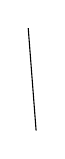
\begin{tikzpicture}\draw (0,0)--(.1,-1.3);\end{tikzpicture}}}

\uline{Théorème de trivialité cohomologique du Frobénius absolu.}
L'hom
\diagram{\begin{tikzcd}[column sep=large,row sep=large]
H^0(X,F) \arrow[d,phantom,"\wr" description] & H^0(X,F)\\
H^0(X,\operatorname{Fr}_{X*}(F)) \arrow[ur,"H^0(\operatorname{Fr}_{F/X})"'] &
\arrow[from=1-1,to=1-2,phantom,"\deleted{\unsure{\longrightarrow}}" description]
\end{tikzcd}}
est l'\uline{identité}, pour $\forall$ faisceau $F$ sur $X_{\text{ét.}}$.
\margin{\figure{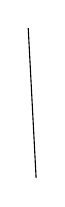
\begin{tikzpicture}\draw (0,0)--(.1,-1.9);\end{tikzpicture}}}

\uline{Corollaire} 1 Si $F$ est un faisceau en groupes,
\diagram{\begin{tikzcd}[column sep=large,row sep=large]
H^1(X,F) \arrow[d,phantom,"\wr" description] & H^1(X,F)\\
H^1(X,\operatorname{Fr}_{X*}(F)) \arrow[ur,"H^1(\operatorname{Fr}_{F/X})"'] &
\end{tikzcd}}
est l'\uline{identité}.

\uline{Corollaire} 2 Si $F^\bullet$ est un \inserted{complexe de} faisceaux \deleted{\unsure{abéliens, des}} \inserted{de $A$-Modules} ($A$ un \deleted{faisceau \unsure{d'anneaux}} \inserted{anneau quelconque}) \inserted{$F^\bullet$ borné sup.}, alors
\diagram{\begin{tikzcd}[column sep=large,row sep=large]
\mathrm R\Gamma_X(F^\bullet) \arrow[d,phantom,"\wr" description] & \mathrm R\Gamma_X(F)\\
\mathrm R\Gamma_X(\operatorname{Fr}_{F^\bullet/X*}(F^\bullet)) \arrow[ur,"\mathrm R\Gamma_X(\operatorname{Fr}_{F^\bullet/X})"'] &
\arrow[from=1-1,to=1-2,phantom,"\deleted{\unsure{\longrightarrow}}" description]
\end{tikzcd}}
est l'\uline{identité} dans la catégorie \inserted{$D(A)$} dérivée de la catégorie des $A$-modules.
En particulier $H^i(X,F)\unsure{\mathbin{-}}H^i(X,F)$ est l'identité.

Ces corollaires résultent du th. en utilisant le calcul de $\mathrm R^1\Gamma_X$ resp. de $\mathrm R\Gamma_X$ par \uline{résolutions}. / Pour prouver le Thm, on note que \deleted{\unsure{si $s$ est une section}} \deleted{\unsure{on conclut par fonctorialité}} l'hom
\diagram{\begin{tikzcd}H^0(X,F) \arrow[r,no head,"H^0(\operatorname{Fr}_{F/X})"] & H^0(X,F)\end{tikzcd}}
est \uline{fonctoriel} en $F$. D'autre part, si $F$ est le faisceau final, c'est l'identité, grâce à la prop. Ces deux faits ensemble donnent \unsure{trivialt} la conclusion.
\mspage{32}

\scanpage{34}
$S$ catégorie avec produits fibrés

$M$ ens de morphismes \unsure{st.bl} par composition, par chgmt de base (m. \unsure{déclarés} étales), d'où pour $\forall X\in\operatorname{Ob}\underline S$, une catégorie $X_{\text{ét}}$.
Sur chaque $X_{\text{ét}}$, on suppose donné une \uline{topologie} \inserted{\unsure{standart|standard}}, de sorte que, \deleted{\unsure{les hom}} pour $\forall$ flèche $f:X\to Y$ dans $S$, le foncteur correspondant
\diagram{\begin{tikzcd}Y_{\text{ét}} \arrow[r,no head,"f^*"] & X_{\text{ét}}\end{tikzcd}}
est ``continu''.

$f$ endom du foncteur identique de $S$. Considérons \deleted{\unsure{les suppos}} les cond

a) Pour $\forall X\in S$, $f_X:X\to X$ induit une équivalence des topos étales,
\[
f_X^*:\widetilde X_{\text{ét}}\longrightarrow\widetilde X_{\text{ét}}
\]
b) Pour $\forall p:X'\to X\in M$, le morphisme canonique $X'\unsure{\mathbin{-}}X'^{(p/S)}$ est un isom, i.e. le carré
\margin{\diagram{\begin{tikzcd}[column sep=large,row sep=large]
X' \arrow[d,"p"'] & X'^{p/X} \arrow[l] \arrow[d] & X' \arrow[l,"\operatorname{Fr}_{X'/X}"'] \arrow[ll,bend right=25,no head,"f_{X'}" above] \arrow[dl,"p"]\\
X & X \arrow[l,"f_X"'] &
\end{tikzcd}}}
\diagram{\begin{tikzcd}[column sep=large,row sep=large]
X' \arrow[d,no head] & X' \arrow[l,"f_{X'}"'] \arrow[d,no head,"p"]\\
X & X \arrow[l,"f_X"']
\end{tikzcd}}
est cartésien

Donc \inserted{b) implique que} le foncteur $f_X^*:X_{\text{ét}}\mathbin{-}X_{\text{ét}}$ est \uline{isomorphe} au foncteur identique, d'où résulte que le morphisme \inserted{de Topos} qu'il induit $\unsure{F_X^*|f_X^*}:\widetilde X_{\text{ét}}\mathbin{-}\widetilde X_{\text{ét}}$ est une équivalence, isomorphe au foncteur identique \deleted{\unsure{par}}, par un isom \uline{unique} \uline{prolongeant} l'isomorphisme donné $F_{-/X}$ sur les faisceaux représentés. Donc b) $\Rightarrow$ a).
\mspage{33}

\scanpage{36}
\deleted{\[
f_X^*\bigl(\unsure{f_X^*}(X')\xrightarrow{\unsure{\operatorname{Fr}_{F/X}^*}}f_X^*(X')\bigr)
\]}
\deleted{$F_{X*}(F$}
\diagram{\begin{tikzcd}[column sep=large,row sep=large]
X' \arrow[d,"p"'] & X'^{p/X} \arrow[l] \arrow[d] & X'\,! \arrow[l,"\sim"',"\exists\text{ isom}" above] \arrow[ll,bend right=35,"f_{X'}" above] \arrow[dl,"p"]\\
X & X \arrow[l,"f_X"'] &
\end{tikzcd}}
\margin{\deleted{\unsure{?}}}
Peut-être que a) implique aussi b), en tous cas c'est vrai si on renforce a) en exigeant que $f_X$ garde la propriété \unsure{dite} après \uline{$\forall$} changement de base (en particulier le chgt de base $f_X:X\mathbin{-}X$ !).

Le prolongt de $\operatorname{Fr}_{X'/X}^*$ \inserted{$(X'\in\operatorname{Ob}X_{\text{ét}})$} aux faisceaux en $\operatorname{Fr}_{F/X}$ se \uline{caractérise}, \inserted{pour $X$ fixé}, par la \unsure{propriété} d'être fonctoriel en $F$ (et d'être un prolongt). Il est évidemment l'identité sur les faisceaux constants :
\diagram{\begin{tikzcd}[column sep=huge]
f_X^*(I_X)=I_X \arrow[r,"\operatorname{Fr}_{F/X}^*","\substack{\Vert\\\mathrm{id}_{I_X}}"'] & I_X
\end{tikzcd}}
comme on voit en se ramenant au cas où $I$ est réduit à un élément. On a \deleted{fonctorialité} compatibilité des $\operatorname{Fr}_{F/X}$ par chgmt de base \uline{quelconques}. La compatibilité aux chgmt de base étales, $+$ fonctorialité en $F$, suffit à le caractériser également -- \deleted{(\unsure{donc indépendance} de la \unsure{topologie} \unsure{de} $f_X$ !!!)}
\margin{\figure{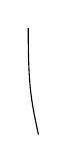
\begin{tikzpicture}\draw (0,0)..controls(0,-.7)and(.03,-.9)..(.13,-1.35);\end{tikzpicture}}}

Il induit l'identité sur les $H^0$, donc sur les $H^i$, $\mathrm R\Gamma_X$ $\cdots$
\mspage{35}

\scanpage{38}
\deleted{\uline{\unsure{Platitude} \unsure{des?}}}

\deleted{\unsure{Variances} pour

\unsure{des|les} $G$-\unsure{f}-\unsure{torseurs}

(\unsure{Groupes} \unsure{réductifs})}
\mspage{37}

\scanpage{39}
\uline{Steinberg}
\mspage{38}

\scanpage{40}
\uline{Brauer--Séveri}

Dans \unsure{Chap} $\overline{\underline{\mathrm{VI}}}$
\mspage{39}

\scanpage{41}
\unsure{\S}\quad\deleted{\uline{Systèmes linéaires et} \unsure{schémas}} \uline{Schémas de Brauer}

\uline{Séveri}

\uline{Déf} \uline{Schéma de Brauer Séveri} \deleted{\unsure{X}} $P/S$ : il devient un fibré projectif loc. fppf

\deleted{\uline{Remarques}}

\uline{Proposition} 1 Un tel $P$ est \uline{projectif} et lisse sur $S$. Le faisceau \deleted{\unsure{\Omega}} $\underline\omega_{X/S}^{-1}$ est ample rel. à $S$.

\uline{Proposition} 2 \deleted{Si $P/S$ a une section, alors $P$} \inserted{Pour que $P$ soit un fibré projectif,} il \uline{\unsure{ft} et suff.} qu'il existe sur $P$ un faisceau inversible \deleted{\unsure{dont les}} de degré 1 sur chaque fibre, ou ce qui revient au $=$, tel que
\[
\underline L^{\otimes(r+1)}\otimes\underline\Omega^r_{X/S}
\]
soit isomorphe à l'image inverse d'un faisceau inv. sur $S$.
\margin{\figure{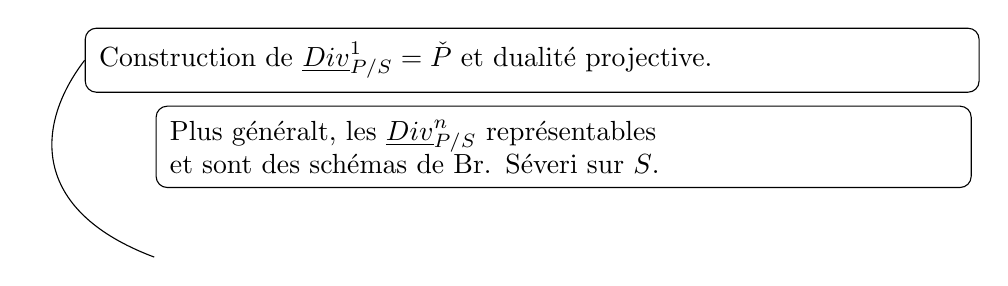
\begin{tikzpicture}[x=1cm,y=1cm]
\node[draw,rounded corners,align=left,text width=11cm,inner sep=5pt] (a) at (0,1.1) {\uline{Construction de} $\underline{\operatorname{Div}}^1_{P/S}=\check P$ et \uline{dualité projective}.};
\node[draw,rounded corners,align=left,text width=10cm,inner sep=5pt] (b) at (.4,0) {Plus généralt, les $\underline{\operatorname{Div}}^{\unsure{n}}_{P/S}$ représentables\par et sont des schémas de Br. Séveri sur $S$.};
\draw (a.west)..controls(-6.3,.3)and(-6.4,-.8)..(-4.8,-1.4);
\end{tikzpicture}}}
\margin{\figure{\begin{tikzpicture}\draw (0,0)--(-.15,0)--(-.15,-2.7)--(0,-2.7);\end{tikzpicture}}}

\unsure{Ca} signifie \unsure{encore} que le résultat de classification donné au $\mathrm N^\circ1$ pour $\operatorname{Pic}(P)$ est valable $\ldots$

\margin{\uline{Corollaire} Cas d'un schéma de base régulier.}

\uline{Proposition} 3 Si $P$ admet une section \inserted{sur $S$}, c'est un fibré projectif : utiliser la théorie de descente \inserted{et dualité des projectifs}.
\margin{\figure{\begin{tikzpicture}\draw (.15,0)--(0,0)--(0,-.8)--(.15,-.8);\end{tikzpicture}}}
\unsure{Évident que aussi} si $\forall$ Module loc. libre sur $S$ est libre (p.ex. $S$ local) \deleted{\unsure{schéma régulier de dim 1} \unsure{spectre} d'un anneau \inserted{principal}}
\mspage{40}

\scanpage{42}
\mspage{-VI-6-}
\hfill n°383

indices $1,\ldots,n$ ; soit $\pi$ la permutation de $\{1,2,\ldots,n\}$ correspondante ; posons $s_i=s_{H_i}$. Notre assertion est vraie dans les cas suivants :

a) $\pi$ est la permutation circulaire $(1,2,\ldots,n)$ : en effet on a
\[
s_2s_3\ldots s_ns_1=s_1^{-1}(s_1s_2\ldots s_n)s_1\ ;
\]

b) $\pi$ est la transposition $(i,i+1)$ de deux indices $i,i+1$ (ici on identifie $1$ et $n+1$) tels que $s_is_{i+1}=s_{i+1}s_i$ ; c'est, en effet, trivial. Notons que la relation $s_is_{i+1}=s_{i+1}s_i$ revient à dire que $H_i$ et $H_{i+1}$ sont perpendiculaires, c'est-à-dire qu'on a $(e_i|e_{i+1})=0$. Donc, d'après le lemme 5 et la prop.1, il existe un couple d'indices $(i,i+1)$ tels que $s_is_{i+1}=s_{i+1}s_i$.

Il reste donc à montrer que le sous-groupe $\underline{T}$ du groupe symétrique $\underline{S}_n$, engendré par la permutation circulaire $(1,\ldots,n)$ et la transposition $(i,i+1)$ est égal à $\underline{S}_n$. Or, comme $(j,j+1)=(1,\ldots,n)(j-1,j)(1,\ldots,n)^{-1}$ (pour $j=1,\ldots,n$ ; on identifie aussi $0$ et $n$), on voit par récurrence que toute transposition de la forme $(j,j+1)$ appartient à $\underline{T}$. D'autre part, pour tout $\pi\in\underline{S}_n$, la permutation $\pi'=(1,2)(2,3)\ldots(\pi(1)-1,\pi(1))\pi$ laisse l'élément $1$ invariant ; ceci démontre, par récurrence sur $n$, que $\underline{S}_n$ est engendré par les transpositions $(j,j+1)$. On a donc bien $\underline{S}_n=\underline{T}$. C.Q.F.D.

Il résulte de la prop.2 que toutes les transformations de \unsure{poulcrier} de $G$ ont le même ordre $h=h(G)$. Ce nombre s'appelle le \uline{nombre de Coxeter} de $G$.
\mspage{41}

\scanpage{43}
\margin{Notion \uline{loc.} \uline{\unsure{triviale}}\unsure{?}}

[\uline{Corollaire} $P$ fibré projectif $\Longleftrightarrow$ $P$ \unsure{adm} loc. une section \inserted{(i.e. est loc. \unsure{trivial})\deleted{\unsure{fibré projectif}}}, et une certaine obstruction dans $H^2(S,\underline{O}_S^*)$ est nulle\ldots]
\margin{en conséquence.}

[\uline{Corollaire} Si $S$ régulier, $P$ fibré projectif ssi il est loc. trivial, ou encore ssi ses fibres génériques le sont.
\margin{\unsure{peut être avec prop 2}}

Autre façon de procéder, valable si $S$ est \uline{strictement \inserted{loc} factoriel} [i.e. tout \uline{schéma} étale dessus est \inserted{loc} factoriel] ----
\figure{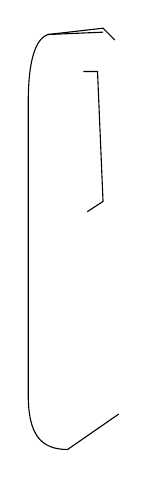
\begin{tikzpicture}[x=1cm,y=1cm]
\draw (0.4,5.1) -- (0.25,5.25) -- (-0.45,5.17) .. controls (-0.65,5.1) and (-0.7,4.7) .. (-0.7,4.3) -- (-0.7,0.6) .. controls (-0.7,0.1) and (-0.55,-0.1) .. (-0.2,-0.1) -- (0.45,0.35);
\draw (-0.45,5.17) -- (0.25,5.2);
\draw (0,4.7) -- (0.18,4.7) -- (0.25,3.05) -- (0.05,2.92);
\end{tikzpicture}}

\uline{Corollaire} \unsure{locale isotrivialité}.
\figure{\begin{tikzpicture}\draw (0,0) .. controls (4,0.15) and (9,0.55) .. (13,0.75);\end{tikzpicture}}

b) \uline{Déf} \uline{Système linéaire} \inserted{\uline{de div. sur} $X/S$}, \uline{paramétré} \uline{par un schéma} $\check{P}/S$ : c'est loc fppf un syst. lin. de div. paramétré par un fibré projectif.
\margin{[$X\to S$ \unsure{fid\textsuperscript{t}} plat loc prés. finie]}
\deleted{Système linéaire}

\deleted{\unsure{Indiquer que}}
Indiquer que $P/S$ est un schéma de Brauer-Séveri.
\margin{\uline{Système linéaire} (tt court).}

classe d'équivalence .....
\mspage{42}

\scanpage{44}
\mspage{-VI-5-}
\hfill n°383

non liés. Comme $a$ est une extrémité de $X$, il existe un indice $i$, par exemple $2$, tel que $a$ ne soit lié à aucun noeud de $X'_i$. On peut alors prendre $X_1=X'_1\cup\{a\}$, $X_2=X'_2$. C.Q.F.D.

On reprend les notations du début.

DEFINITION 2.- \uline{On appelle graphe de} $G$ \uline{un graphe dont les noeuds sont les murs} $H_1,\ldots,H_n$ \uline{de} $C$, \uline{deux éléments} $H_i$ \uline{et} $H_j$ $(i\ne j)$ \uline{étant liés si et seulement si} $(e_i|e_j)\ne0$.

Comme $G$ opère transitivement sur ses chambres (§3, n°1, prop.1), les graphes de $G$ sont tous isomorphes.

Supposons $G$ essentiel. Soit $G=G_1\times\ldots\times G_s$ la décomposition de $G$ en produit de groupes irréductibles. Le graphe $X$ de $G$ est isomorphe à la somme disjointe des graphes $X_i$ des $G_i$. Pour que $G$ soit irréductible, y faut et y suffit que son graphe $X$ soit connexe.

PROPOSITION 1.- \uline{Le graphe} $X$ \uline{de} $G$ \uline{est une forêt}. \uline{Si} $G$ \uline{est irréductible}, \uline{ce graphe est un arbre}.

En effet, en vertu du lemme 5, $X$ n'admet pas de circuit.

3. \uline{Définition des transformations de Coxeter}.

Appelons \uline{chambre ordonnée} relative à $G$ la donnée d'une chambre $C$ et d'une indexation $(H_1,\ldots,H_n)$ de ses murs par $1,2,\ldots,n$.

DEFINITION 3.- \uline{On appelle transformation de Coxeter définie par une chambre ordonnée} $C$, $(H_1,\ldots,H_n)$ \uline{l'élément} $s_{H_1}s_{H_2}\ldots s_{H_n}$ \uline{de} $G$.

PROPOSITION 2.- \uline{Toutes les transformations de Coxeter de} $G$ \uline{sont conjuguées dans} $G$.

Soient $c$ et $c'$ deux transformations de Coxeter. Comme $G$ opère transitivement sur les chambres (§3, n°1, prop.1), on est ramené au cas où elles sont définies par la même chambre sous-jacente $C$, et où elles ne diffèrent donc que par l'ordre des
\mspage{43}

\scanpage{45}
\uline{Relations} a) Morphismes $X\longrightarrow\unsure{\check{\check{P}}|\check{P}}$ et syst. lin. de div \unsure{sans pts fixes paramétrés} par $P$.

\deleted{Applications}
b) Syst. lin. de div. ``\unsure{str.}'' sans ``p. fixe'' paramétré par $\check{P}$, et applications rationnelles sur $S$
\[
X\longrightarrow\check{P}
\]
avec \unsure{petite} propriété supplémentaire \uline{de nature locale}
\margin{[qui est inutile si $X$ est régulier \deleted{\illegible{1}} ou strict loc. factoriel]}

c)
\[
\underline{\mathrm{Syst.lin}}_{X/S}\xrightarrow{\lambda}\underline{\mathrm{Pic}}_{X/S}
\]
morphisme naturel : (\unsure{ayant} \unsure{d'ailleurs} une section canonique). Si $X/S$ est propre à fibres géom. intègres, alors $\lambda$ est rel. représentable comme la grassmannienne complète d'un schéma de Brauer-Séveri généralisé (Attention, il y a une question d'effectivité des données de descente dans un fibré projectif relatif un Module non loc. libre !].

Si, au lieu de fibres géom. intègres, on suppose $f_*(O_X)\simeq O_S$ \unsure{univ\textsuperscript{t}}, on trouve encore un morphisme représentable par un \uline{ouvert} d'un fibré \deleted{projectif} de Brauer-Séveri généralisé .....
\margin{\uline{\unsure{à vérifier}}\par
\unsure{Montrer}\par
$X\to S$ est \uline{projectif}\par
si $S$ hensélien local à fibres \unsure{géoréd!}\par
si $\unsure{q}(\unsure{\mathrm{Pic}}(X/S))$\par
est \uline{loc} \unsure{noéthérien}}
\mspage{44}

\scanpage{46}
\mspage{-VI-4-}
\hfill n°383

par des figures, en associant à chaque noeud un point du plan, et en joignant deux points par un arc si les noeuds correspondants sont liés. On saute le laius pontifiant sur la nature non-mathématique des figures.
\figure{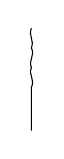
\begin{tikzpicture}\draw (0,1.3) .. controls (-0.04,1.2) and (0.04,1.15) .. (0,1.05) .. controls (0.05,0.95) and (-0.04,0.9) .. (0,0.8) .. controls (-0.04,0.7) and (0.05,0.65) .. (0,0.55) -- (0,0);\end{tikzpicture}}

Un graphe $X'$ est un \uline{sous-graphe} de $X$ si $X'\subset X$ et si deux noeuds de $X'$ liés dans $X'$ sont liés dans $X$. On dit que $X'$ est un sous-graphe \uline{plein} si, de plus, deux noeuds de $X'$ qui sont liés dans $X$ sont liés dans $X'$.

Un noeud $a$ d'un graphe $X$ est dit une \uline{extrémité} de $X$ si $a$ est lié à au plus un noeud distinct de $a$.

On dit qu'un graphe $X$ est \uline{connexe} s'il n'existe aucune partition $X=X'\cup X''$ de $X$ telle qu'aucun élément de $X'$ ne soit lié à aucun élément de $X''$.

Un graphe fini $X$ s'appelle un \uline{circuit} s'il a au moins $3$ noeuds, et si ces noeuds peuvent être indexés $a_1,\ldots,a_n$ $(n\geqslant3)$ de sorte que les simplexes de $X$ soient $(a_1,a_2)$, $(a_2,a_3)$,\ldots,$(a_{n-1},a_n)$,$(a_n,a_1)$ ; un circuit n'admet aucune extrémité. Un graphe dont aucun sous-graphe n'est un circuit s'appelle une \uline{forêt}. Une forêt connexe s'appelle un \uline{arbre}.

LEMME 6.- \uline{Toute forêt finie non vide} $X$ \uline{admet une extrémité}.

Prenons $a_1\in X$. Construisons, par récurrence, une suite $(a_1,\ldots,a_i,\ldots)$ d'éléments de $X$ telle que $a_i$ soit lié à $a_{i-1}$ et $a_{i+1}$ et que $a_{i+1}$ soit distinct de $a_{i-1}$ (pour $i\geqslant2$). Les $a_i$ sont distincts car, \inserted{sinon,} $X$ contiendrait un circuit. La suite $(a_i)$ est donc finie. Son dernier terme est évidemment une extrémité de $X$.

LEMME 7.- \uline{Soit} $X$ \uline{une forêt finie ayant au moins deux noeuds}. \uline{Il existe une partition} $X=X_1\cup X_2$ \uline{telle que deux noeuds distincts appartenant à un même} $X_i$ \uline{soient non-liés}.

On raisonne par récurrence sur $\operatorname{card}(X)$, le cas $\operatorname{card}(X)=2$ étant trivial. Soit $a$ une extrémité de $X$ (lemme 6), et $X'$ le complémentaire de $a$, muni de la structure de sous-graphe plein de $X$. Alors $X'$ est une forêt ; d'après l'hypothèse de récurrence on a une partition $X'=X'_1\cup X'_2$ telle que deux noeuds appartenant à un même $X'_i$ soient
\mspage{45}

\scanpage{47}
Donc $\underline{\mathrm{Syst.lin.div}}_{X/S}$ est représentable ssi $\underline{\mathrm{Pic}}_{X/S}$ l'est.

\uline{Donnons nous} un syst. linéaire paramétré par $\check{P}/S$ de Br. Sév., et considérons la section correspondante $\xi$ de $\underline{\mathrm{Pic}}_{X/S}$.
\diagram{\begin{tikzcd}[column sep=large,row sep=large]
\underline L \arrow[d,phantom] & \underline L\otimes_S O_{\check P}(1)\otimes\underline N \arrow[d,phantom] \\
X \arrow[r,no head]\arrow[d,no head] & X\times_S\check P\arrow[d,no head] \\
S \arrow[r,no head] & \check P
\end{tikzcd}}

Je dis que $\xi$ \uline{est représentable par un $\underline L$ inversible sur $X$} \uline{ssi} \uline{$\check P$ est un fibré projectif}.
\margin{[$f:X\to S$ propre, $f_*(O_X)=O_S$ \unsure{univ\textsuperscript{t}}]}

Car la condition est suffisante \inserted{(\unsure{on sait par construction} $\unsure{\mathcal L}$ de $\xi$)}, prouvons qu'elle est nécessaire. \deleted{\unsure{Alors}} En effet, on a alors un Module de prés. finie $Q$ sur $S$, et un \inserted{mono}morphisme $\check P\longrightarrow P(Q)$, je dis que c'est un isom sur un $P(E)$, où $E$ est un quotient loc. libre de $Q$. Ce est par descente, avec le $=$ \unsure{principe} ---

\margin{Il suffit\par
$f_*(O_X)\simeq O_S$\par
et $f$ \deleted{\unsure{plat}} \inserted{de prés. finie}}

\margin{Si $X/S$ \unsure{adm} une section il est trivial que $\check P$ est ``trivial'', \unsure{car alors tout diviseur} \unsure{trivial} sur $X$ .....}
\figure{\begin{tikzpicture}\draw (0,2.6) -- (0,0.3) .. controls (0,0.05) and (0.12,0) .. (0.5,0);\end{tikzpicture}}

\uline{Remarque} Partant d'un Br. Sév. \unsure{non trivial}, on construit un $\xi$ ne provenant pas d'un $\underline L$ \unsure{au} $=$ \unsure{relation d'incidence can.}
\mspage{46}

\scanpage{48}
\mspage{-3-}
\hfill n°379

COROLLAIRE.- \uline{Soient} $A$ \uline{un anneau principal}, $M$ \uline{un} $A$-\uline{module divisible}. \uline{Alors}, \uline{pour toute suite exacte} $E'\longrightarrow E\longrightarrow E''$ \uline{d'applications} $A$-\uline{linéaires la suite} :
\[
\operatorname{Hom}(E'',M)\longrightarrow\operatorname{Hom}(E,M)\longrightarrow\operatorname{Hom}(E',M)
\]
\uline{est exacte}.

Même démonstration que dans la prop. 1 de la rédaction.

\uline{Remarque}.- Nous étudierons plus tard, sous le nom de \uline{modules injectifs}, les modules, (sur un anneau quelconque), vérifiant le corollaire.

Le reste de la rédaction est inchangé.

\begin{center}\unsure{-:-:-:-}\end{center}
\figure{\begin{tikzpicture}\draw (0,0) -- (0.18,-0.01);\end{tikzpicture}}
\mspage{47}
